%%%%%%%%%%%%%%%%%%%%%%%%
%
% $Autor: Wings $
% $Datum: 2020-07-24 09:05:07Z $
% $Pfad: GDV/Vortraege/latex - Ausarbeitung/Kapitel/Einleitung.tex $
% $Version: 4732 $
%
%%%%%%%%%%%%%%%%%%%%%%%%

\chapter{Portenta Vision Shield}


The Arduino Portenta Vision Shield is an add-on board providing machine vision capabilities and additional
connectivity to the Portenta family of Arduino boards, designed to meet the needs of industrial automation. The
Portenta Vision Shield connects via a high-density connector to the Portenta boards with minimal hardware and software setup, refer figure ~\ref{VisionShield1}. \cite{arduinoVisionShield:2024}

\begin{figure}
	\begin{center}
		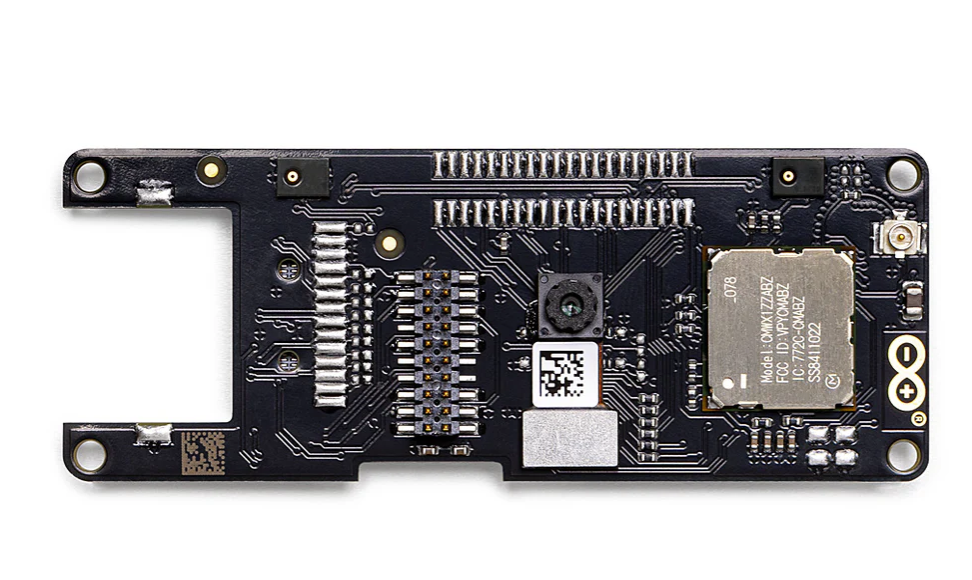
\includegraphics[width=0.7\linewidth]{Images/VisionShield/VisionShield.png}
		\caption{Portenta Vision Shield}
		\label{VisionShield1}
	\end{center}
\end{figure}



\section{Key Features}

\begin{itemize}
	\item \textbf{Onboard Camera}:
	
	\textbf{Himax HM-01B0 Camera Module}
	\begin{itemize}
		
		\item Ultra-Low-Power Image Sensor designed for always-on vision devices and applications
		\item Window, vertical flip, and horizontal mirror readout
		\item Programmable black level calibration target, frame size, frame rate, exposure, analog gain (up to 8x), and digital gain (up to 4x)
		\item Automatic exposure and gain control loop with support for 50 Hz / 60 Hz flicker avoidance
		\item Motion Detection circuit with programmable ROI and detection threshold with digital output to serve as an interrupt
		
		\textbf{Supported Resolutions:}
		
		\item QQVGA (160x120) at 15, 30, 60, and 120 FPS 
		\item QVGA (320x240) at 15, 30, and 60 FPS \cite{arduino_datasheet:2025}
	\end{itemize}

	\item \textbf{Onboard Microphone}: Dual ultra-compact, low-power, omnidirectional, digital MEMS microphones (MP34DT06J)
	\item \textbf{Connectivity}:
	\begin{itemize}
		\item LoRa Module (CMWX1ZZABZ-078) for the LoRa variant (SKU: ASX00026)
		\item RJ45 Connector for Ethernet capabilities in the Ethernet variant (SKU: ASX00021)
	\end{itemize}
	\item \textbf{External Memory}: Onboard microSD card slot
	\item \textbf{Dimensions}: 66.04 x 25.40 mm
	\item \textbf{Weight}: 8 g \cite{arduino_datasheet:2025}
\end{itemize}


\begin{figure}
	\begin{center}
		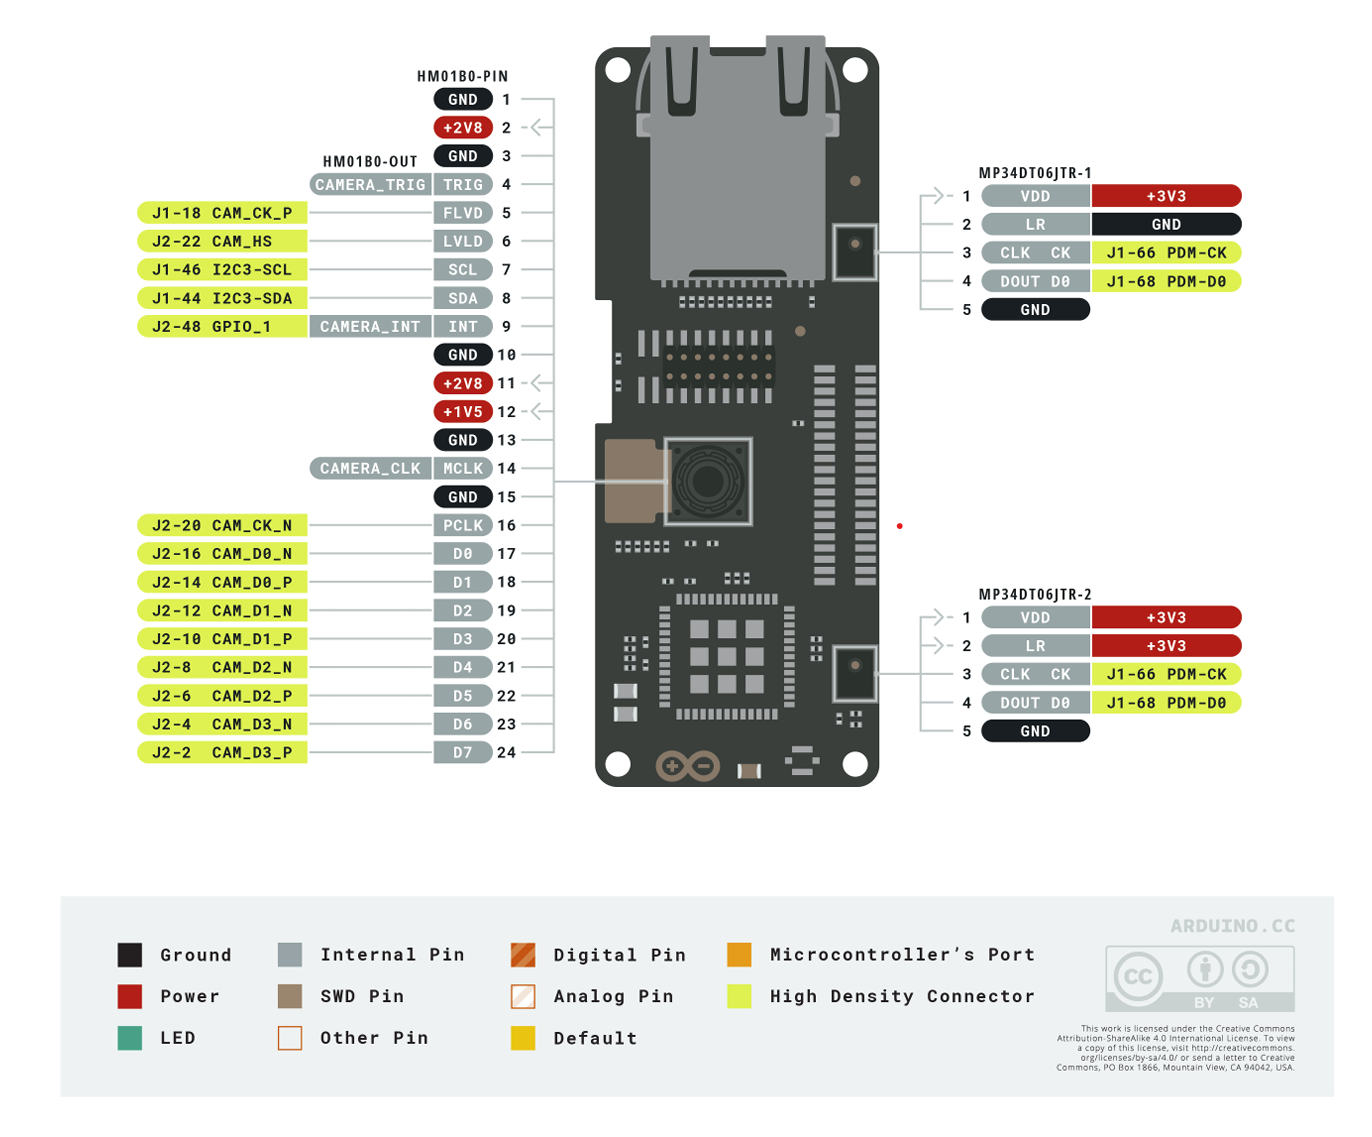
\includegraphics[width=0.7\linewidth]{Images/VisionShield/PinDiagram.png}
		\caption{Portenta Vision Shield PinDiagram}
		\label{PinDiagram} \cite{arduino_datasheet:2025}
	\end{center}
\end{figure}



\section{Hardware Components}

The LoRa implementation in the Portenta Vision Shield comprises several essential hardware components(Refer figure ~\ref{tab:general-specifications}) that work together to enable seamless communication, data handling, and energy management. Below are the key components:  \cite{arduino_portenta:2025}.

\begin{figure}
	\begin{center}
		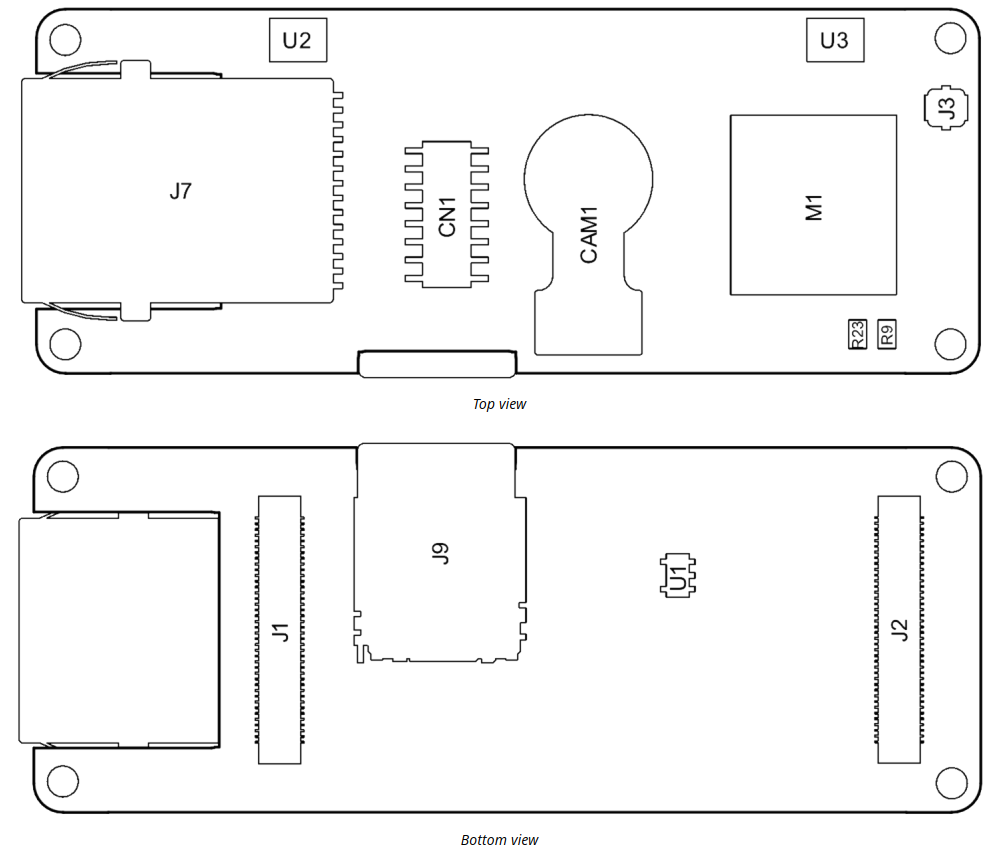
\includegraphics[width=0.7\linewidth]{Images/VisionShield/BoardTopology.png}
		\caption{Board}
		\label{BoardTopology}
	\end{center}
\end{figure}

\subsection{LoRa Transceiver Module}
\begin{itemize}
	\item \textbf{Function:} Provides radio communication using LoRa modulation for sending and receiving data \cite{semtech_sx1276:2025}.
	\item \textbf{Integrated Module:} Murata CMWX1ZZABZ module based on Semtech SX1276 transceiver \cite{murata_transceiver:2025}.
	\item \textbf{Features:} Supports configurable frequency bands (868 MHz and 915 MHz), spreading factors, and adaptive data rates \cite{semtech_sx1276:2025}.
\end{itemize}

\subsection{Microcontroller Unit (MCU)}
\begin{itemize}
	\item \textbf{Function:} Serves as the core processor for managing data, interfacing with sensors, and handling communication protocols .
	\item \textbf{MCU in Portenta H7:} Dual-core architecture with an ARM Cortex-M7 (480 MHz) and Cortex-M4 (240 MHz) .
	\item \textbf{Features:} High processing power, low energy consumption, and extensive I/O support for peripheral devices \cite{arduino_portenta:2025}.
\end{itemize}

\subsection{Antenna}
\begin{itemize}
	\item \textbf{Function:} Facilitates the transmission and reception of LoRa signals \cite{semtech_lora:2025}.
	\item \textbf{Antenna Type:} External antenna connected via a U.FL connector for enhanced signal quality \cite{murata_transceiver:2025}.
	\item \textbf{Considerations:} Designed for optimal frequency compatibility and communication range \cite{semtech_lora:2025}.
\end{itemize}

\subsection{Power Supply}
\begin{itemize}
	\item \textbf{Function:} Provides power to the Vision Shield and its components, ensuring energy efficiency .
	\item \textbf{Sources:} Compatible with the Portenta H7’s onboard power supply and external batteries .
	\item \textbf{Components:} Includes voltage regulators to maintain stable operation and extend battery life \cite{arduino_portenta:2025}.
\end{itemize}

\subsection{Sensors and Peripherals}
\begin{itemize}
	\item \textbf{Function:} Collects environmental data and enhances functionality for specific applications .
	\item \textbf{Examples:} Integrated camera for vision applications, microphones for audio input. .
	\item \textbf{Interface:} Communicates with the MCU using I2C, SPI, or UART protocols \cite{arduino_portenta:2025}.
\end{itemize}

\subsection{Memory}
\begin{itemize}
	\item \textbf{Function:} Stores firmware, application data, and communication logs \cite{arduino_portenta:2025}.
	\item \textbf{Memory in Portenta H7:} Flash memory for non-volatile storage and SRAM for temporary processing tasks \cite{arduino_portenta:2025}.
	\item \textbf{Capacity:} 16 MB of NOR Flash and 8 MB of SDRAM, providing ample space for advanced applications \cite{arduino_portenta:2025}.
\end{itemize}

\begin{figure}
	\begin{center}
		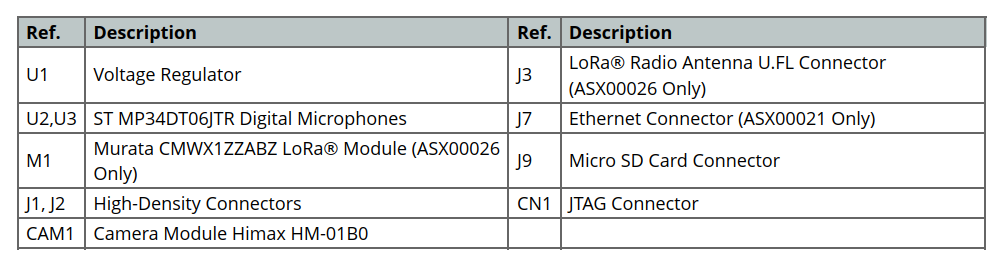
\includegraphics[width=0.7\linewidth]{Images/VisionShield/Discription.png}
		\caption{Board Topology}
		\label{BoardTopology}
	\end{center}
\end{figure}

<<<<<<< Updated upstream
\section{Application Examples}
\begin{itemize}
	\item \textbf{Industrial Automation}:
	\begin{itemize}
		\item Quality control: Automatically detect product defects in production lines.
		\item Predictive maintenance: Monitor equipment for early signs of wear or failure.
		\item Automated sorting: Sort items based on color, shape, or size in conveyor systems.\cite{arduino_datasheet:2025}
	\end{itemize}
	\item \textbf{Surveillance}:
	\begin{itemize}
		\item Real-time threat detection: Identify and alert authorities of potential threats.
		\item Perimeter surveillance: Detect intrusions or breaches in perimeter security.
	\end{itemize}
	\item \textbf{Machine Vision and Edge Computing}:
	\begin{itemize}
		\item Smart agriculture: Monitor crops and soil conditions for issues like pest infestations or nutrient deficiencies.
		\item Autonomous vehicles: Enhance navigation and obstacle detection.
		\item Robotics: Enable robots to see and interpret their surroundings for complex tasks.
	\end{itemize}
	\item \textbf{Audio Analysis and Sound-Based Applications}:
	\begin{itemize}
		\item Acoustic monitoring: Detect anomalies or predict maintenance needs based on machinery noise patterns.
		\item Voice-activated systems: Enable voice commands for hands-free control.
		\item Anomaly detection: Detect unusual sounds like breaking glass or alarms in security systems. \cite{arduino_datasheet:2025}
	\end{itemize}
\end{itemize}

\begin{comment}
	
	\section{Power}
	
	The Portenta H7/C33 supplies 3.3 V power to the LoRa module (ASX00026 only), Ethernet communication (ASX00021 only), Micro SD slot, and dual microphones via the 3.3 V output of the high-density connectors. An onboard LDO regulator supplies a 2.8 V output (300 mA) for the camera module.
	
	\section{Camera Module}
	
	The Himax HM-01B0 Module is a very low-power camera with 324x324 resolution and a maximum of 60 FPS depending on the operating mode. Video data is transferred over a configurable 8-bit interconnect with support for frame and line synchronization. The module delivered with the Portenta Vision Shield is the monochrome version. Configuration is achieved via an I2C connection with the compatible Portenta boards microcontrollers.
	
	HM-01B0 offers very low-power image acquisition and provides the possibility to perform motion detection without main processor interaction. The “Always-on” operation provides the ability to turn on the main processor when movement is detected with minimal power consumption.
	
	\textbf{Note:} The Portenta C33 is not compatible with the camera of the Portenta Vision Shield.
	
	\section{Digital Microphones}
	
	The dual MP34DT05 digital MEMS microphones are omnidirectional and operate via a capacitive sensing element with a high (64 dB) signal-to-noise ratio. The microphones have been configured to provide separate left and right audio over a single PDM stream.
	
	The sensing element, capable of detecting acoustic waves, is manufactured using a specialized silicon micromachining process dedicated to produce audio sensors.
	
	\section{Micro SD Card Slot}
	
	A Micro SD card slot is available under the Portenta Vision Shield board. Available libraries allow reading and writing to FAT16/32 formatted cards.
	
	\section{Ethernet (ASX00021 Only)}
	
	Ethernet connector allows connecting to 10/100 Base TX networks using the Ethernet PHY available on the Portenta board.
>>>>>>> Stashed changes


\section{First Step with Portenta Vision Shield:}

\subsection{Getting Started With the Portenta Vision Shield Camera}
This tutorial shows you how to capture frames from the Arduino Portenta Vision Shield Camera module and visualize the video output through a Processing sketch. ~\ref{VisionShield} \cite{portentaVisionShieldCamera:2024}
	\begin{figure}
		\begin{center}
			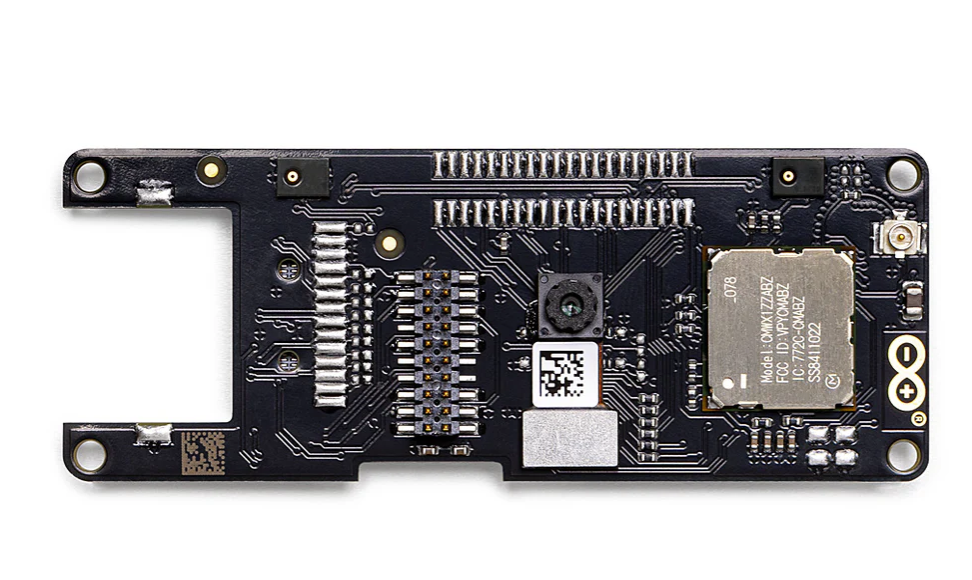
\includegraphics[width=0.7\linewidth]{Images/VisionShield/VisionShield.png}
			\caption{VisionShield}
			\label{VisionShield}
		\end{center}
	\end{figure}

\subsection{Goals:}
\begin{itemize}
	\item Capturing the frames from the camera
	\item Sending the frames as a byte stream through a Serial connection
	\item Visualising the frames in Processing
\end{itemize}

\subsection{Required Hardware and Software:}
\begin{itemize}
	\item Portenta H7
	\item Portenta Vision Shield (LoRa or Ethernet)
	\item USB-C cable
	\item Arduino IDE 2.3.2
	\item Processing software
\end{itemize}
\subsection{Instructions:}
	Accessing the Portenta Vision Shield's camera data is done with the help of both Arduino and the Processing IDE. The Arduino sketch handles the capture of image data by the on-board camera, while the java applet created with Processing helps to visualize this data with the help of a serial connection. The following steps will run you through how to capture, package the data through the serial port and visualize the output in Processing.
\begin{itemize}
	\item \textbf{The Basic Setup:} Connect the Portenta Vision Shield to your Portenta H7 as shown in the figure. The top and bottom high density connecters are connected to the corresponding ones on the underside of the H7 board. Plug in the H7 to your computer using the USB-C cable. ~\ref{Connection VS}
	\begin{figure}
		\begin{center}
			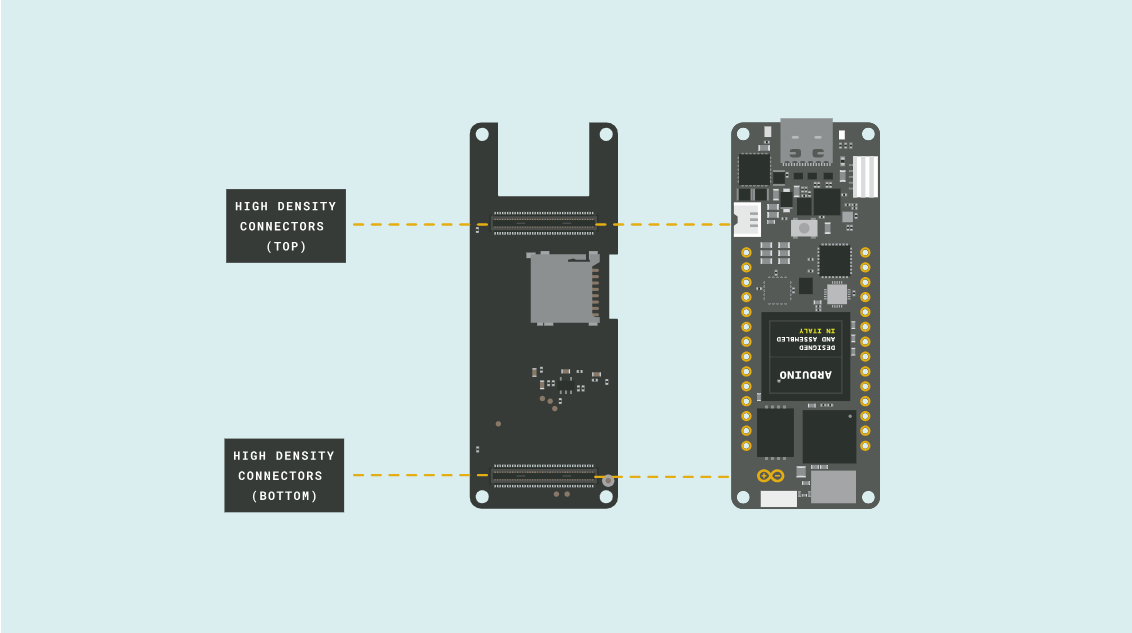
\includegraphics[width=0.7\linewidth]{Images/VisionShield/Connection VS.png}
			\caption{Connection VS}
			\label{Connection VS}
		\end{center}
	\end{figure}
	\item \textbf{Adding the Portenta to the List of Available Boards:} In your Arduino IDE, open the board manager and search for "portenta". Find the Arduino mbed-enabled Boards library and click on "Install" to install the latest version of the mbed core (1.2.3 at the time of writing this tutorial). ~\ref{Portentaport}
	\begin{figure}
		\begin{center}
			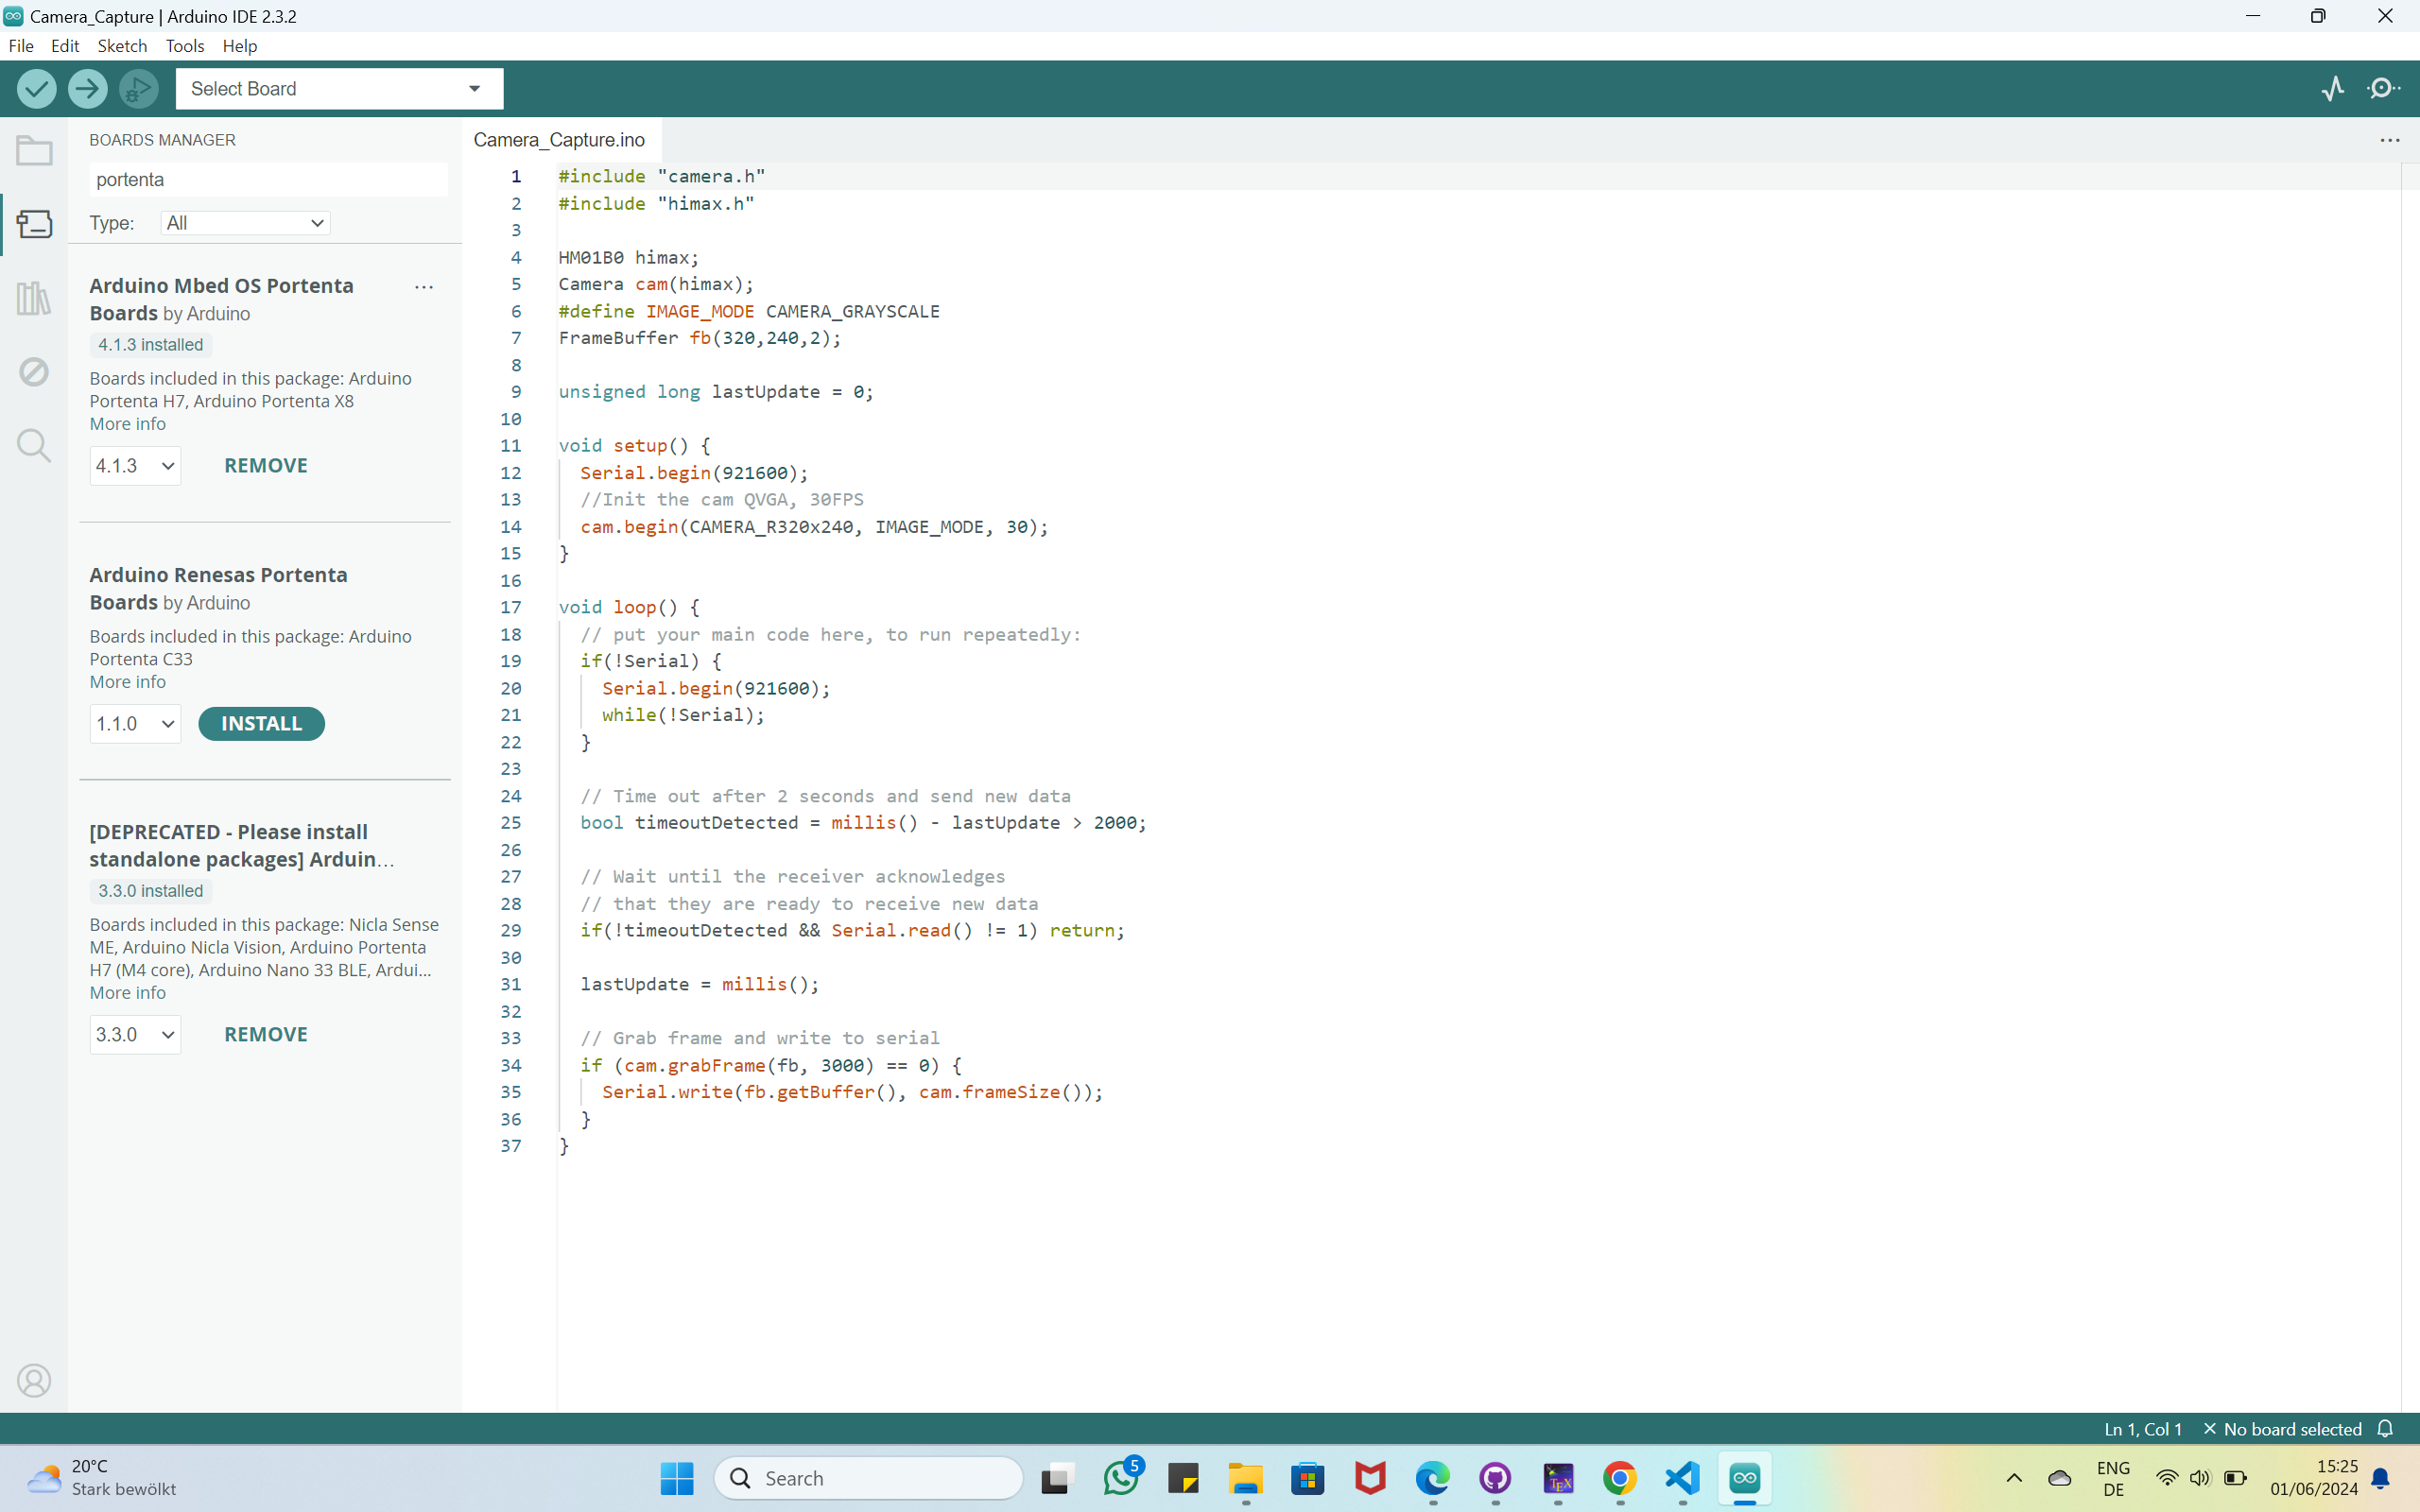
\includegraphics[width=0.7\linewidth]{Images/PortentaH7/Portentaport.png}
			\caption{Portentaport}
			\label{Portentaport}
		\end{center}
	\end{figure}
	
	\item \textbf{Uploading the Classic Blink Sketch:} Let's program the Portenta with the classic blink example to check if the connection to the board works. 
	
	\begin{lstlisting}
		// the setup function runs once when you press reset or power the board
		void setup() {
			// initialize digital pin LED_BUILTIN as an output.
			pinMode(LED_BUILTIN, OUTPUT);
			digitalWrite(LED_BUILTIN, HIGH); // turn the LED off after being turned on by pinMode()
		}
		
		// the loop function runs over and over again forever
		void loop() {
			digitalWrite(LED_BUILTIN, LOW); // turn the LED on (LOW is the voltage level)
			delay(1000); // wait for a second
			digitalWrite(LED_BUILTIN, HIGH); // turn the LED off by making the voltage HIGH
			delay(1000); // wait for a second
		}   
		
	\end{lstlisting}
	
\end{itemize}

\end{comment}